\documentclass[10pt, a4paper]{article}
\usepackage{graphicx, listings}

\author{Emil Boesgaard Nørbjerg, emno@itu.dk}
\date{\today}
\title{Documentation of assignment 00}

\begin{document}
\maketitle
On figure \ref{fig:IsLeapYear}, a flowchart diagram of the method \verb!IsLeapYear! is shown.
The method belongs to the \verb!MyApp! namespace, and the \verb!Program! class.
The purpose of the method is to determine whether or not a given year is a leap year.

From the domain, and the requrements we know have the following definition for a leap year:
\begin{quote}
    The leap year function should only apply to years from 1582.
    Every year that is exactly divisible by four is a leap year, except for years that are exactly divisible by 100, but these centennial years are leap years if they are exactly divisible by 400. 
    For example, the years 1700, 1800, and 1900 are not leap years, but the years 1600 and 2000 are.
\end{quote}

This gives rise to the program descriped in figure \ref{fig:IsLeapYear}.
A design decision is that since any year before 1582 is ill defined for leap years, the method throws an error in that case.

The method operates by using modulo, to determine if the year is divisible by 100, 400, and 4, or none of them.
As descriped the year is a leap year, if it devides 4, or 100 and 400. 
Otherwise it is not a leap year. 

\begin{figure}[htbp]
    \centering
    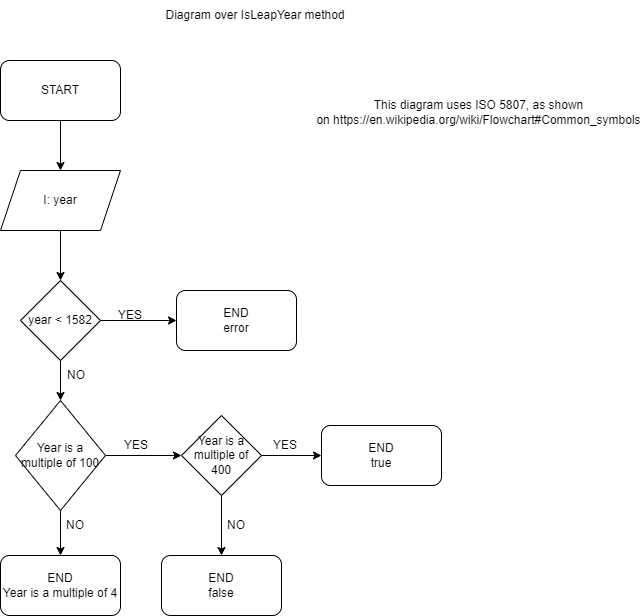
\includegraphics[width=0.7\textwidth]{pic/LeapDocu.png}
    \caption{Flowchart of IsLeapYears implementation}
    \label{fig:IsLeapYear}
\end{figure}

\begin{lstlisting}[caption="Listing of c\# code"]
public static bool IsLeapYear(int year){
    if(year < 1582 ){
        throw new ArgumentException();
    }

    if (year % 100 == 0){
        if(year % 400 == 0){
            return true;
        }
        return false;
    }
    return year % 4 == 0;
}
\end{lstlisting}
\end{document}